\chapter{Coupling Majorana Mode to a Double Quantum Dot }
%--------------------------------------------------------------------------
\Jesus{This section is still a bit disorganized since most of the results are new.   }
In this section we present the results for the NRG analysis of the Anderson model applied to the case of a Double Quantum Dot (DQD) attached to a Majorana mode (See \ref{fig:GeneralModel}). Extending the  Hamiltonian \eqref{eq:QD-Mham} to a coupling with a DQD we obtain the following general Hamiltonian:   

\begin{equation}
H =\sum_{i=1}^2\sum_{k,\sigma}\left(\epsilon_{i}+\frac{U_i}{2}\right)d_{\sigma}^{\dagger}d_{i\sigma}+ \frac{U_i}{2}(d_{i \sigma}^{\dagger}d_{i \sigma}-1)^{2} + t_i(\gamma d_{+,\dw}+d^\dagger_{+,\dw}\gamma) + V_id^\dagger_{i\sigma}c_{k\sigma}+V_i^* c^\dagger_{k\sigma}d_{i\sigma}.
\label{General model}
\end{equation}

\Jesus{I neglected $\epsilon_M$ in this case. Depending on the future NRG results I will choose to add it or leave it that way. }


\begin{figure}[h]
\centering
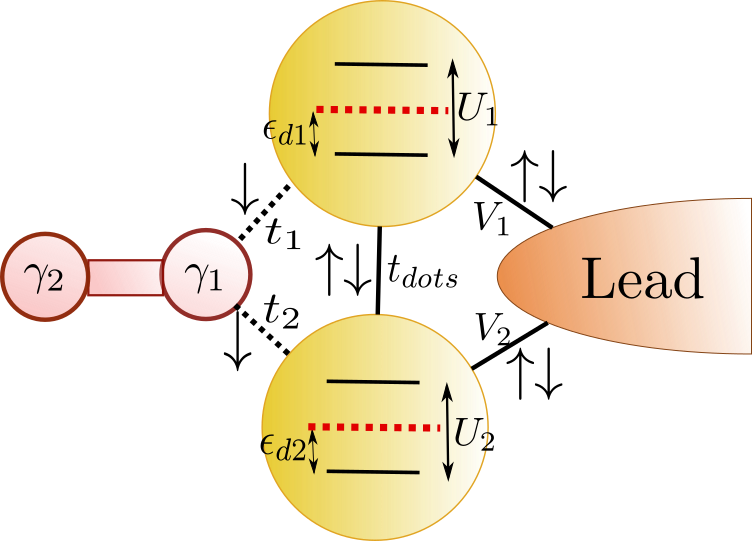
\includegraphics[scale=0.4]{IMAGES/GenModel.png}
\caption{\label{fig:GeneralModel}General model.} 
\end{figure}



In order to understand the physical properties of this model, we probed a set of thought processes. The main variable in this analysis is the Density of States.  We  will observe its evolution on both QDs under the tuning of the model parameters such as:
\begin{enumerate}
    \item Hopping between Dots and Majorana Mode ($t_1 , t_2$). 
    \item Gate voltage ($\ed{1} , \ed{2} $)
    \item Inter dot coupling ($t_{dots}$)
\end{enumerate}


These processes intend to show whether it is possible to "manipulate" the majorana modes inside the dots by tuning the established parameters. The number of possible combinations of parameters is actually pretty huge. We used ballistic transport tho predict which one of them show interesting physics. Those models where also treated with the NRG approach in the interacting case. The process we selected are summarized in \ref{fig:Models}. 

To built the ballistic transport graph (See \ref{sec:GraphMethod}) we just need to think that our model is actually merging the DQD graph (\ref{fig:graphDQD}) with the Majorana (Figure \ref{fig:green-M-QD}.b)). No need to write the green transport equations . Note  in graph $\MDQD$ that the  green function  $\Green{d_{1\downarrow},d_{1\downarrow}^{\dagger}}{\MDQD}$  is composed by the greeen function of the DQD $\left(\GreenG{d_{1\downarrow},d_{1\downarrow}^{\dagger}}{\GDQD } \right)$ and the extra term added by the presence of the majorana opperator $f_\downarrow$. In the equations this is simply 

\begin{equation}
    \GreenG{d_{1\downarrow},d_{1\downarrow}^{\dagger}}{\MDQD}=\left[\left(\GreenG{d_{1\downarrow},d_{1\downarrow}^{\dagger}}{\GDQD } \right)^{-1}+\frac{\omega}{\omega+\epsilon_{M}}\frac{E_{d_{1\dw}f_{\dw}}^{\MDQD}}{\left[\GreenG{f_{\downarrow},f_{\downarrow}^{\dagger}}{\MDQD-d_{1}}\right]^{-1}}\right]^{-1}.
\end{equation}
where 
\begin{equation}
    E_{d_{1\dw}f_{\dw}}^{\MDQD}=\left(t_{1}+t_{2}\frac{\left(t_{dots}+\sum_{\mathbf{k}}\frac{V_{1}V_{2}^{*}}{\omega-\epsilon_{\mathbf{k}}}\right)}{\omega-\epsilon_{2}-\sum_{\mathbf{k}}\frac{V_{2}V_{2}^{*}}{\omega-\epsilon_{\mathbf{k}}}}\right)\left(t_{1}^{*}+t_{2}^{*}\frac{\left(t_{dots}^{*}+\sum_{\mathbf{k}}\frac{V_{1}^{*}V_{2}}{\omega-\epsilon_{\mathbf{k}}}\right)}{\omega-\epsilon_{2}-\sum_{\mathbf{k}}\frac{V_{2}^{*}V_{2}}{\omega-\epsilon_{\mathbf{k}}}}\right).
\end{equation}
\Jesus{This fact is difficult to explain. I will need more plots and writing the appendix. For now I will leave here some results}

We then need to compute $\GreenG{f_{\downarrow},f_{\downarrow}^{\dagger}}{\MDQD-d_{1}}$ . This graph is much simple. The neighborhood of  $f_{\downarrow}$ in graph ${\MDQD-d_{1}}$ are $d_2$ (above) and the inverted DQD(bellow). These neighbors are disconnected, hence we can include the in the green function independently. The term above is simply the dot $d_{2\downarrow}$ connected with the lead . 
\begin{equation}
    \frac{\frac{\omega}{\omega+\epsilon_{M}}\left\Vert t_{2}\right\Vert ^{2}}{\omega-\epsilon_{2}-\sum_{\mathbf{k}}\frac{V_{2}V_{2}^{*}}{\omega-\epsilon_{\mathbf{k}}}}.
\end{equation}

 
The term generated by the connection of $f_{\downarrow}$  with the inverted $DQD$ is a bit more complicated. First we need to include the term given by the connection with  $d_{2\downarrow}^\dagger$ which is 

The other term is the contact with the DQD which can be expressed as 
\begin{equation}
    \GreenG{f_{\downarrow},f_{\downarrow}^{\dagger}}{\MDQD-d_{1}}=\left[\omega-\epsilon_{M}-\frac{\frac{\omega}{\omega+\epsilon_{M}}\left\Vert t_{2}\right\Vert ^{2}}{\omega-\epsilon_{2}-\sum_{\mathbf{k}}\frac{V_{2}V_{2}^{*}}{\omega-\epsilon_{\mathbf{k}}}}-\frac{\frac{\omega}{\omega+\epsilon_{M}}\left\Vert t_{2}\right\Vert ^{2}}{\omega+\epsilon_{2}-\sum_{\mathbf{k}}\frac{V_{2}V_{2}^{*}}{\omega+\epsilon_{\mathbf{k}}}}-\frac{\omega}{\omega+\epsilon_{M}}\frac{E_{f_{\dw}d_{1\dw}^\dagger}^{\MDQD-d_1}}{\left[\GreenG{d_{1\downarrow}^{\dagger},d_{1\downarrow}{\dagger}}{\MDQD-d_{1}-f_{\downarrow}}\right]^{-1}}\right]^{-1}.
\end{equation}
Now, note that that graph $\MDQD-d_{1}-f_{\downarrow}$ is actually a double quantum dot with negated couplings. Hence  $\GreenG{d_{1\downarrow}^{\dagger},d_{1\downarrow}{\dagger}}{\MDQD-d_{1}-f_{\downarrow}}$  satisfies the equation \eqref{eq:solGreen} but with variables $-t_{dots}, -t_1 , -t_2, -\ed{1}  , -\ed{2}$


\begin{figure}[H]
\centering
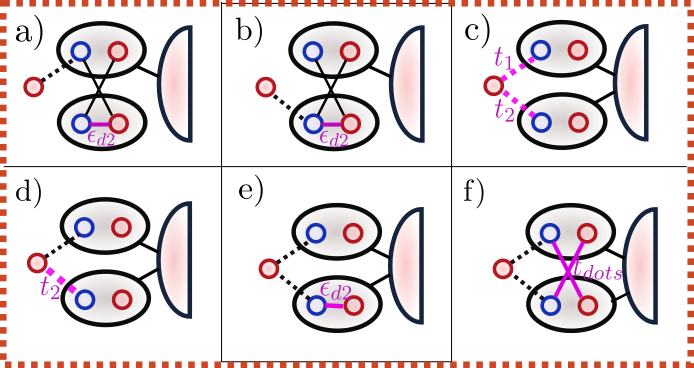
\includegraphics[scale=0.4]{IMAGES/Graphs/Models.png}
\caption{\label{fig:Models}Selected Models .} 
\end{figure}

\begin{figure}[H]
\centering
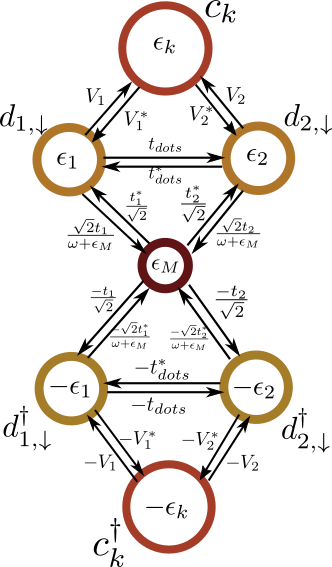
\includegraphics[scale=0.60]{IMAGES/Graphs/DQD-Majorana.png}
\caption{\label{fig:Graph-MDQD} Graph $\MDQD$ representing ballistic transpor through a DQD coupled to a Majorana mode. } 
\end{figure}



\newpage


% -------------------------------------------------------------
\subsection{ a) Removing Kondo and Majorana with QD-interference \label{sec:tdots}}

\begin{figure}[hbt]
\centering
\includegraphics[scale=0.35]{IMAGES/}
\caption{\label{fig:2D/Shift_t1=t2} }
\end{figure}


% -------------------------------------------------------------
\subsection{ b) Indirect Majorana after Removing Kondo with QD-interference \label{sec:tdots}}



\begin{figure}[hbt]
\centering
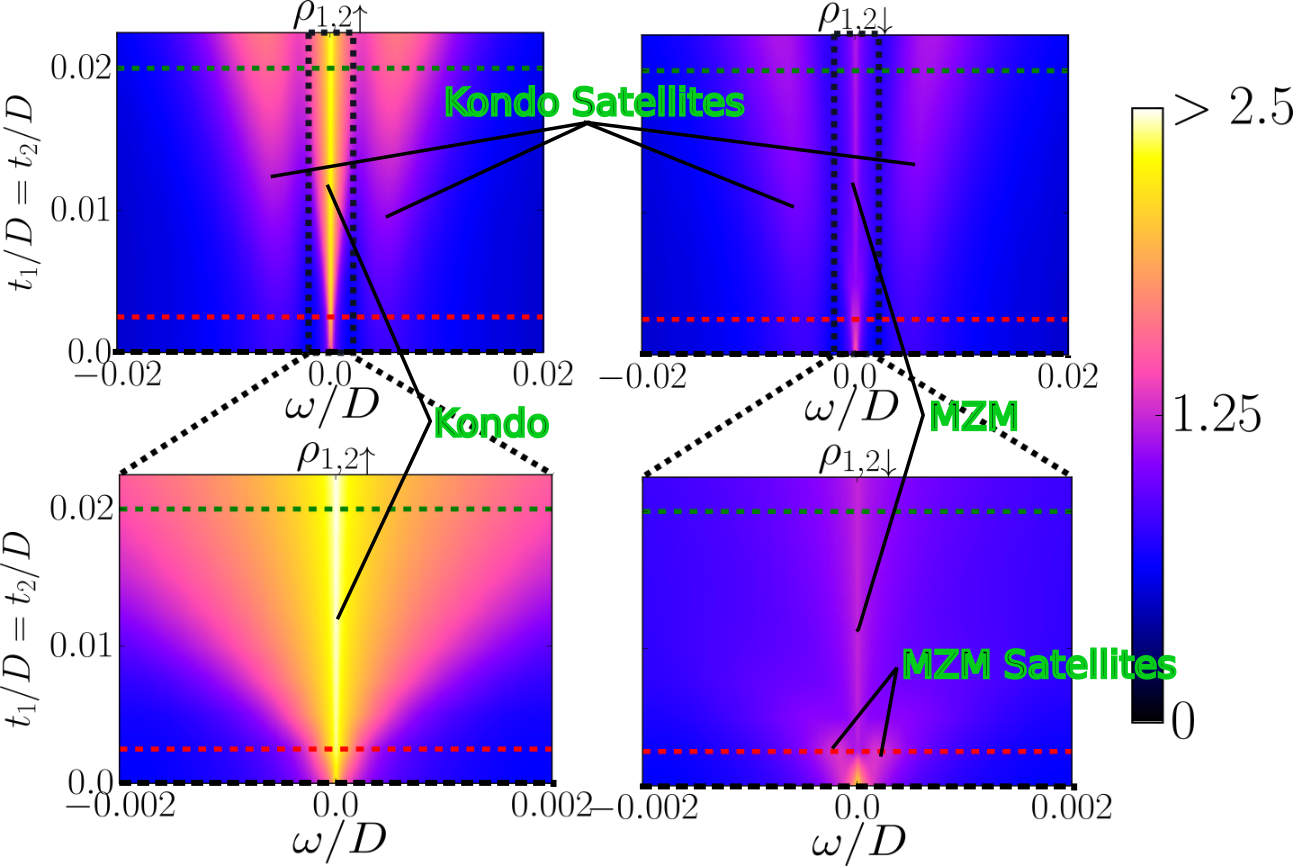
\includegraphics[scale=0.35]{IMAGES/t1=t2/2D.png}
\caption{\label{fig:2D/Shift_t1=t2} Evolution of the DOS of both QDs through $t_1 = t_2$ tuning. UP: Energy scale $\omega \sim 10^{-2}D$. DOWN: Energy scale $\omega \sim 10^{-3}D$. LEFT: Spin $\up$. RIGHT: Spin $\dw$.}
\end{figure}





% -------------------------------------------------------------------
\subsection*{c) Attaching the Majorana mode to the DQD (Tuning $t_1=t_2$) \label{sec:t1=t2}}

\textbf{Parameters:}

$$\Gamma \sim 2.83*10^{-2}D, t_{dots}=0 , U_{1,2} = -2\ed{1,2} = 0.5$$
$$t_1=t_2 \in [0\  ,\  2.5*10^{-2}D]$$

\begin{figure}[hbt]
\centering
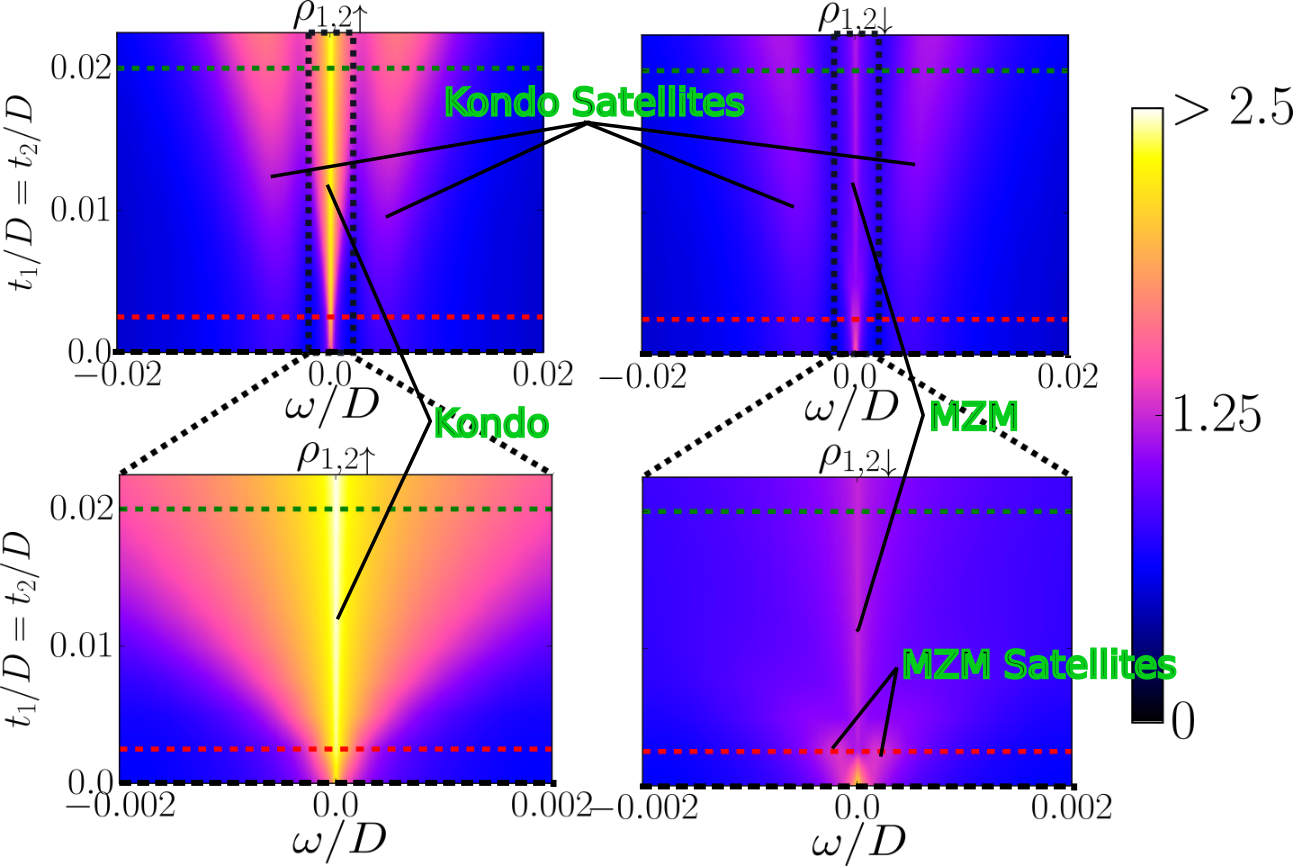
\includegraphics[scale=0.35]{IMAGES/t1=t2/2D.png}
\caption{\label{fig:2D/Shift_t1=t2} Evolution of the DOS of both QDs through $t_1 = t_2$ tuning. UP: Energy scale $\omega \sim 10^{-2}D$. DOWN: Energy scale $\omega \sim 10^{-3}D$. LEFT: Spin $\up$. RIGHT: Spin $\dw$.}
\end{figure}



The first process consists in attaching the Majorana mode to both Quantum Dots symmetrically. For this, we scale up the coupling parameter $t_1=t_2$ from $0$ (Decoupled) to $0.02$ (Completely coupled).The other parameters where chosen with an equilibrium between the dot energy and Coulomb repulsion $(\ed{1,2}=-\frac{U_{1,2}}{2})$  and  without inter-dot coupling $t_{dots}=0$. These circumstances guarantee that the system preserves Particle Hole Symmetry (PHS). Thus the Density of States (DOS) of particles and holes remains equal at all instances $(\rho(-\omega) = \rho(\omega))$. \\

\begin{figure}[hbt]
\centering
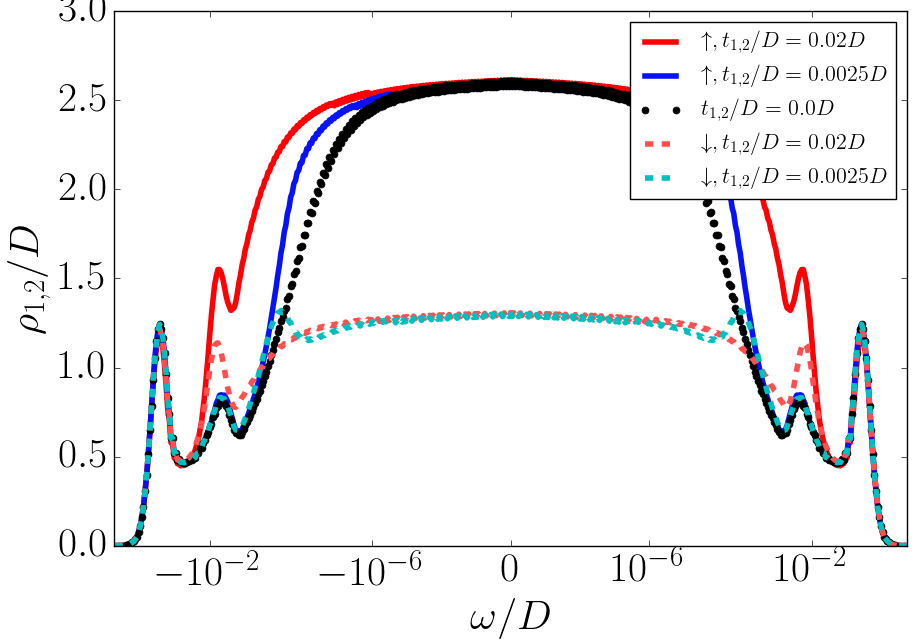
\includegraphics[scale=0.35]{IMAGES/t1=t2/LogPlot.png}
\caption{\label{fig:t1=t2/logplot} Density of states at each QD of the horizontal dashed cuts in \ref{fig:2D/Shift_t1=t2}. The energy is in logarithmic scale.  For $t_1=t_2>0$ spin-$\up$ and spin-$\dw$ DOS split near the order of $\vert \omega \vert \sim t_1,2 $. At the Fermi energy $(\omega =0)$  $\rho_\up = 2\rho_\dw$ due to the presence of the MZM in both QDs. }
\end{figure}

In the case where the majorana is detached from the DQD $(t_1 =t_2 = 0)$, the system favors the appearance of a three-peak at low energies as it is shown in \ref{fig:t1=t2/logplot} . The central peak is produced only by the Kondo effect and the two other satellite peaks are the result of a strong correlation between both dots caused by the indirect exchange of quantum states through the Lead \ref{sec:DoublePeak}. \\

Once the MZM the spin-$\up$ and spin-$\dw$ DOS split at low energies due to the new spin-$\dw$ transport channel through the Majorana mode. The spin-$\dw$ DOS at the Fermi energy ($\omega =0$) decays to the half of the spin-$\up$ DOS $\rho_\dw = \frac{\rho_\up}{2} $. By symmetry in the dot parameters this event occurs equally for both QDs. We adopt this fact as a Majorana signature. Hence we obtain that the MZM leaks inside both quantum dots. 

There is also an additional effect caused by the indirect exchange between the QDs through the Majorana mode . The consequences of this effect depend on the energy range of the majorana couplings $t_1=t_2$.  : 
\begin{enumerate}
    \item If $t_1=t_2 \ll \Gamma $ two more satellites are formed at very low energies ($\sim t_1$) in the spin-$\dw$ DOS (See  \ref{fig:2D/Shift_t1=t2} Spin-down $\omega \sim 10^{-3}D$ ). (See  \ref{fig:2D/Shift_t1=t2} Spin $\up$, $\omega \sim 10^{-3}D$ ).
    \item If $t_1=t_2 \sim \Gamma$ , the MZM contributes to the the growth of the spin-up satellites in the DOS. This effect produces the splitting between the spin-up and spin-down DOS.   (See  \ref{fig:2D/Shift_t1=t2} Spin-$\dw$, $\omega \sim 10^{-2}D$).
\end{enumerate}









% At low energies $(\omega/D \sim 10^{-2})$ \ref{fig:2D/Shift_t1=t2} shows the emergence of a 3-peak in the DOS close to the Fermi energy. This 3-peak is formed by a central peak defined by the Kondo (spin $\up$) and the Majorana (spin $\dw$) peaks. The other two peaks are generated by an indirect exchange of the states between the quantum dots through the leads (SEE ABSTRACT). At even lower energies $(\omega/D \sim 10^{-4})$ it is possible to appreciate the emergence of another 3-peak in the spin down DOS which is present only for small values of the Majorana coupling constants $t_1 = t_2 \ll 0.01D$ (See  \ref{fig:t1=t2/logplot}). These sided peaks are caused by the indirect exchange between both dots through the Majorana Mode. When the Majorana couplings achieve the same order of the dot-lead coupling $\Gamma$ $(t_1 = t_2 \sim  0.01D)$ both sided peaks are merged causing the extinction of the majorana side-peaks and the increase of the indirect exchange peaks at $(\omega/D \sim 10^{-2})$. 

% \begin{figure}[H]
% \centering
% 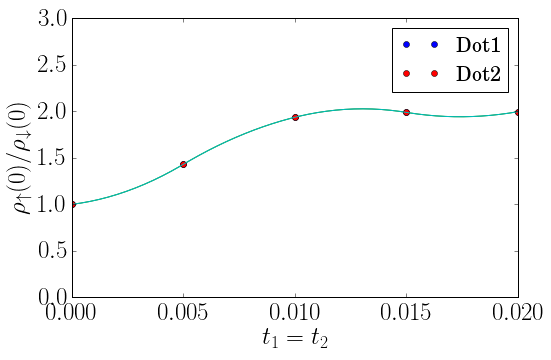
\includegraphics[scale=0.4]{Plots/MSig/Shift_t1=t2.png}
% \caption{\label{fig:MSig/Shift_t1=t2} Relation between the Zero-peaks at the fermi level. The Majorana signature is related to $\frac{\rho_\up(0)}{\rho_\up(0)}=2$.}
% \end{figure}










%--------------------------------------------------------------------

\subsection{ e) Transferring the MZM through gate voltage shifting $\ed{2}$. \label{sec:e2}}

\textbf{Parameters:}

$$\Gamma \sim 2.83*10^{-2}D, t_{dots}=0 , U_{1,2} = -2\ed{1} = 0.5 , t_1=t_2=0.0025$$
$$\ed{2} \in [-0.25 \  , -0.05]$$

This process starts with the DQD coupled symmetrically  to the Majorana mode, just as in \ref{sec:t1=t2}. The idea of this process is to break PHS by increasing the energy of the second QD $\ed{2}$. This procedure should induce the Majorana to tunnel only into the first dot. 


\begin{figure}[h]
\centering
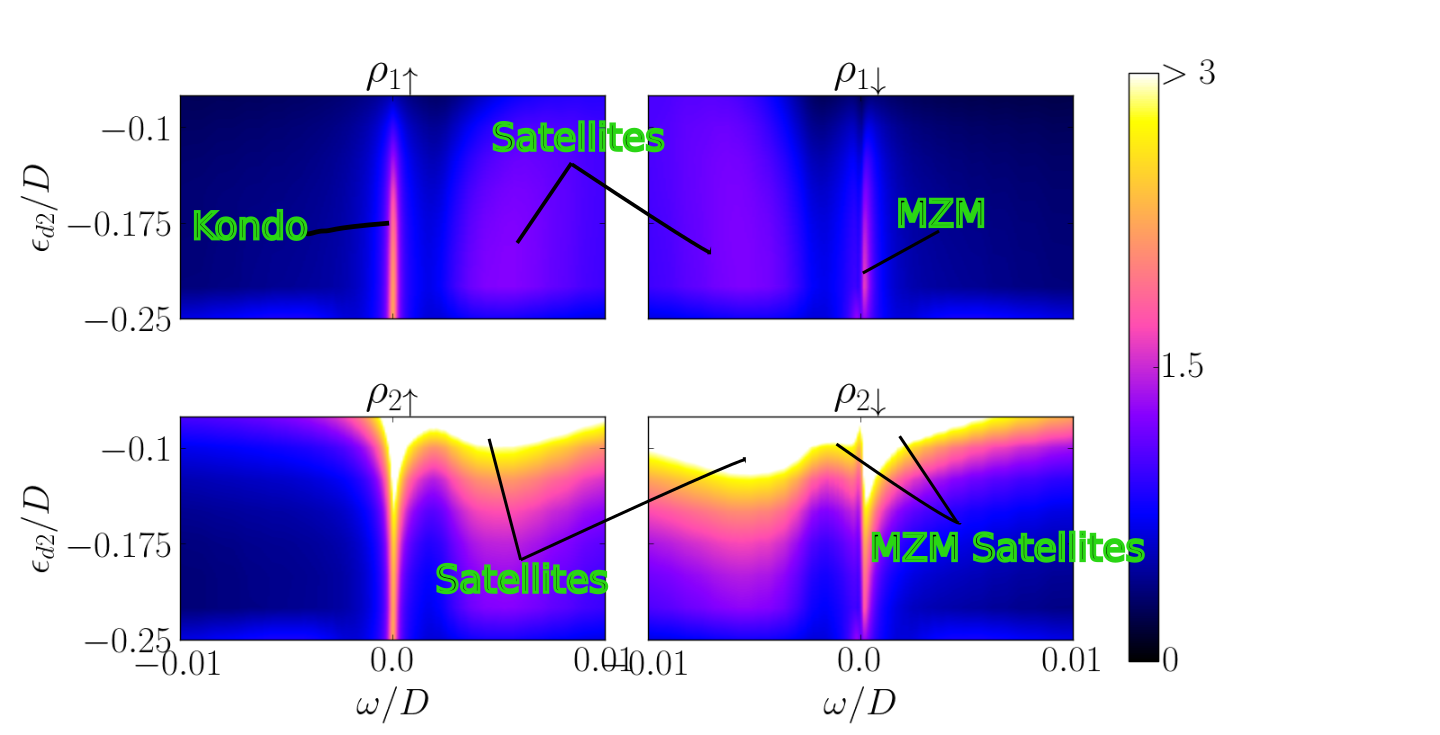
\includegraphics[scale=0.35]{IMAGES/ed2/2D.png}
\caption{\label{fig:2D/Shift_ed2} Evolution of the DOS of both QDs through the $\ed{2}$ tuning. UP: QD1. DOWN: QD2. LEFT: Spin $\up$. RIGHT: Spin $\dw$.}
\end{figure}


In \ref{fig:2D/Shift_ed2} we observe that both, the Kondo and the MZM peaks are preserved in the first QD as well as the majorana signature (See \ref{fig:ed2/Fermi}) when $\ed{2}$ is scaled up to $-0.1$.  However,  PHS breaking will favor the growth of the spin-$\up$ hole $(w>0)$  satellite and the spin-$\dw$ particle $(w<0)$ satellite.




In the second QD the DOS increases abruptly for both spins.The majorana signature is rapidly when  lost . Hence, with this set-up it is actually possible to induce the Majorana to preferably tunnel QD1 in despite of QD2.  \\
\begin{figure}[H]
\centering
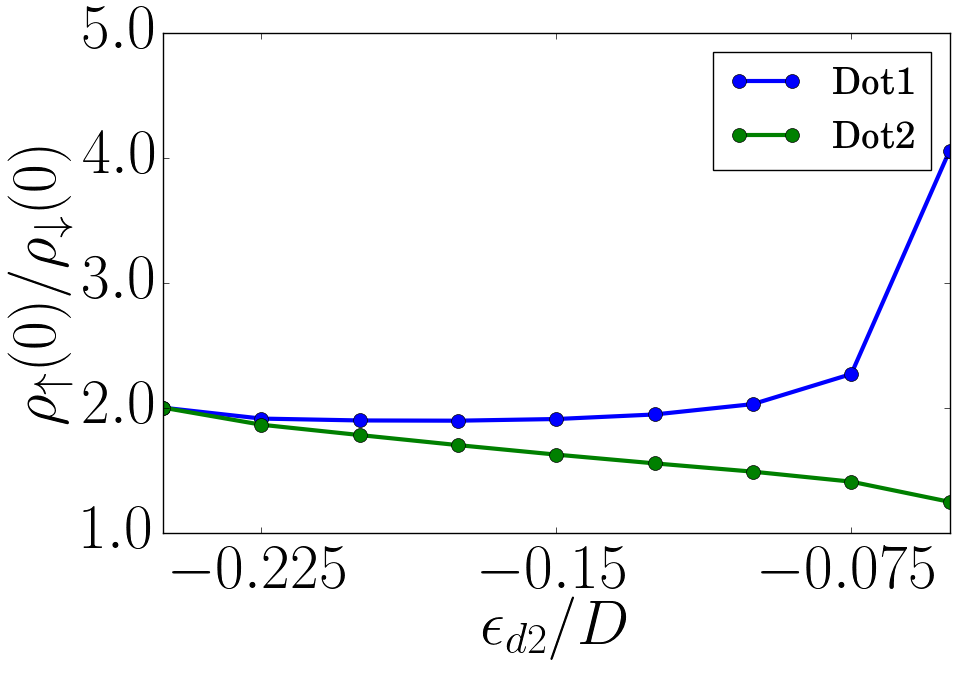
\includegraphics[scale=0.3]{IMAGES/ed2/Fermi.png}
\caption{\label{fig:ed2/Fermi} As described in \ref{sec:t1=t2} the relation $\frac{\rho_\up(0)}{\rho_\up(0)}=2$ constitutes a Majorana Signature . This picture evaluates shows the evolution of the relation $\frac{\rho_\up(0)}{\rho_\up(0)}$ for both QDs. While QD2 losses rapidly the Majorana signature, QD1 maintains it till $\ed{2}\sim -0.1$.}
\end{figure}


\newpage


%---------------------------------------------------------------------------

\section{Particle-Hole symmetric shifting of $\ed{2}=\frac{U}{2}$.}

\begin{figure*}[h]
\centering
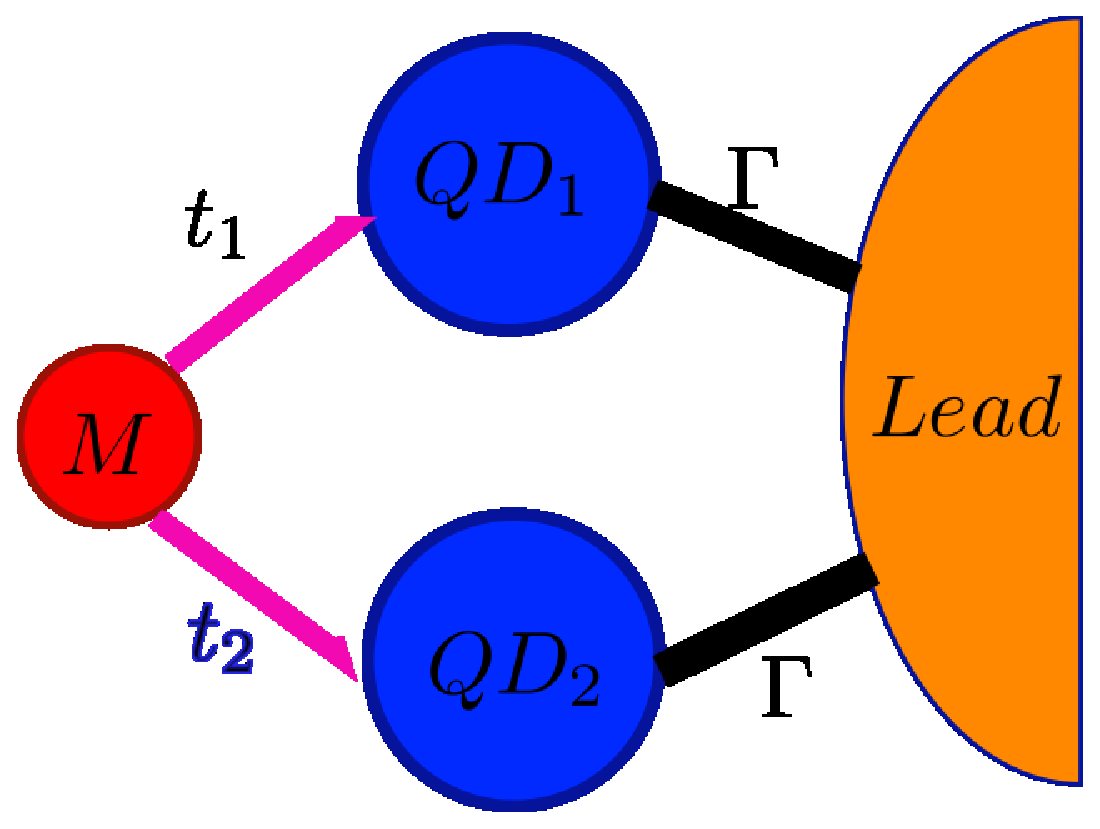
\includegraphics[scale=0.2]{Plots/Model/Majorana-2QD.eps}
\caption{\label{fig:Mod/PHS-Shift_e2.png}$U_{1}=-2\ep_{d1}=0.5$, $\Gamma_{1}=\Gamma_{2}$,
$t_{1}=t_2=0.02$. Variable $\ep_{d2} =\frac{U_{2}}{2}$}
\end{figure*}
\begin{figure}[hbt]
\centering
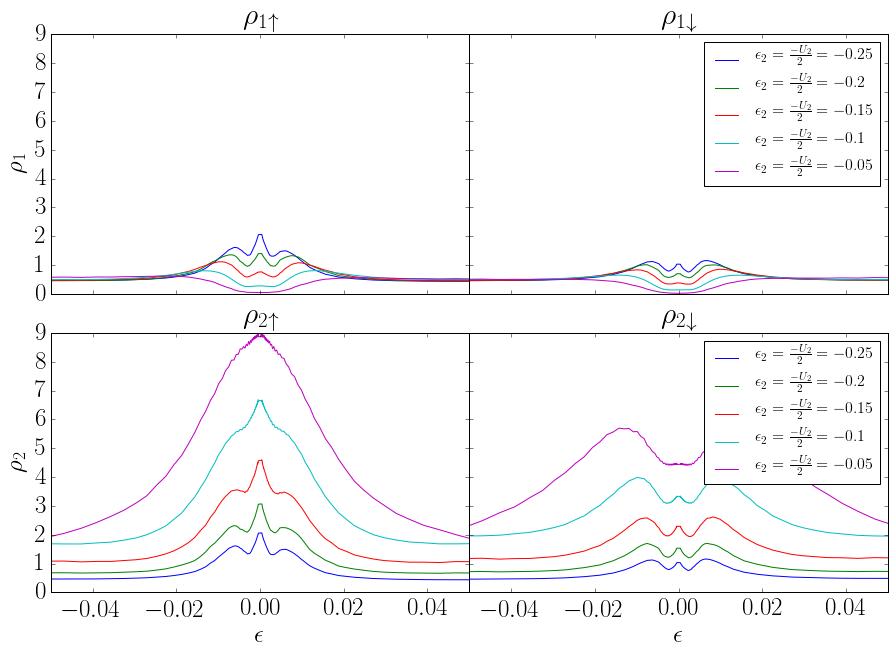
\includegraphics[scale=0.38]{Plots/DOS/PHS-Shift_e2.png}
\caption{\label{fig:DOS/PHS-Shift_e2.png} Evolution of the QDs' DOS for the model in \ref{fig:Mod/PHS-Shift_e2.png} }
\end{figure}
We start again with the symmetric model with both QDs coupled to the Majorana mode, but this time the evolution is performed over $\ep_2=\frac{U}{2}$, such that the model is always Particle-Hole symmetric. This situation is very different from the previous model (\ref{sec:e2}) since the decaying of $U2$ 
equalizes the effect of increasing the dot energy. In \ref{fig:DOS/PHS-Shift_e2.png} we observe that the DOS of QD2 increases while the QD1's DOS decreases, just as it happened in \ref{sec:e2} . However, the Majorana signature remains at $2$ for both dots (See \ref{fig:MSig/PHS-Shift_e2}), meaning that the Majorana is not preferably induced to tunnel to any QD despite the lose of symmetry in the dot energy.

\begin{figure}[hbt]
\centering
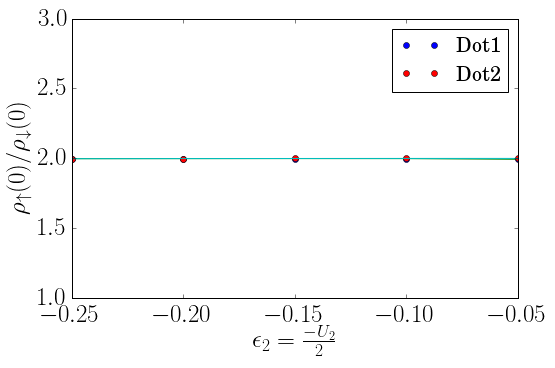
\includegraphics[scale=0.4]{Plots/MSig/PHS-Shift_e2.png}
\caption{\label{fig:MSig/PHS-Shift_e2} Relation between the spin up-down Zero-peaks at the Fermi level. The Majorana signature is related to $\frac{\rho_\up(0)}{\rho_\up(0)}=2$.}
\end{figure}

%---------------------------------------------------------------------------
\section{Shifting $t_2$}

%$U_{1}=U_{2}=-2\epsilon_{d1}=-2\epsilon_{d2}=0.5$, %$\Gamma_{1}=\Gamma_{2}$,
%$t_{1}=0.02$

\begin{figure*}[h]
\centering
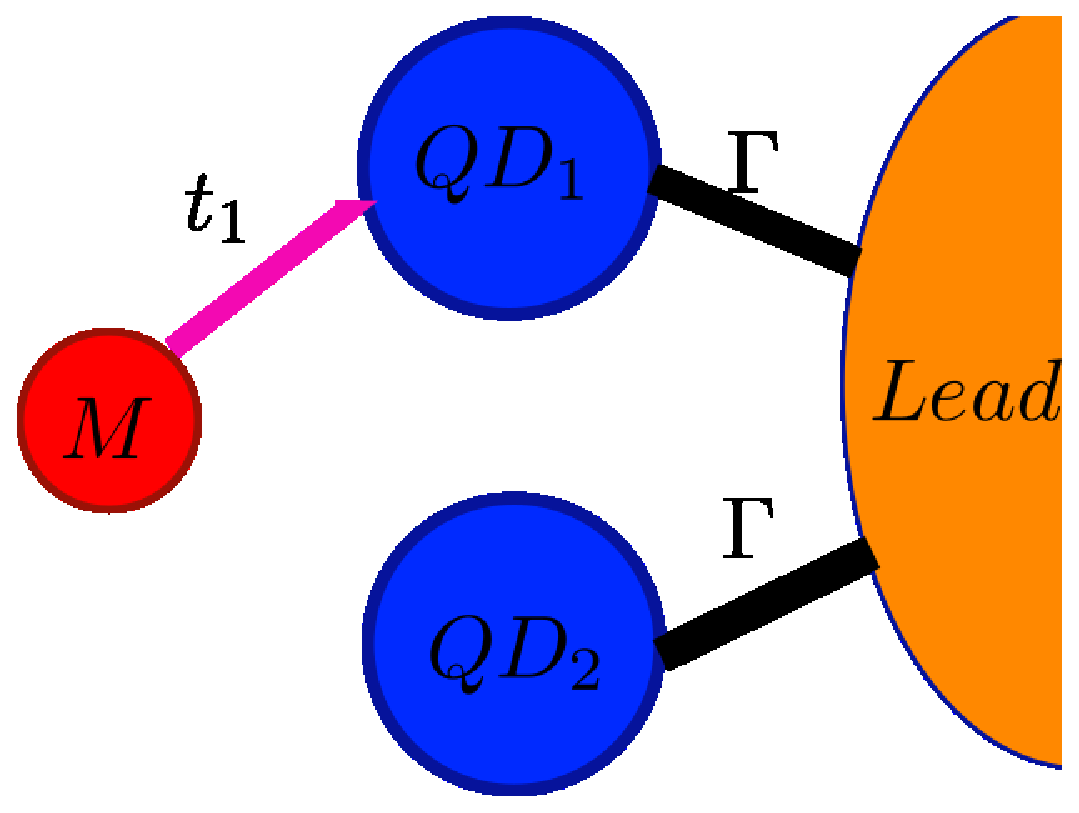
\includegraphics[scale=0.2]{Plots/Model/Majorana-1QD.eps}
\caption{\label{fig:Mod/Shift_t2}$U_{1}=U_{2}=-2\ep_{d1}=-2\epsilon_{d2}=0.5$, $\Gamma_{1}=\Gamma_{2}$,
$t_{1}=0.02$. Variable $t_2$}
\end{figure*}


\begin{figure}[hbt]
\centering
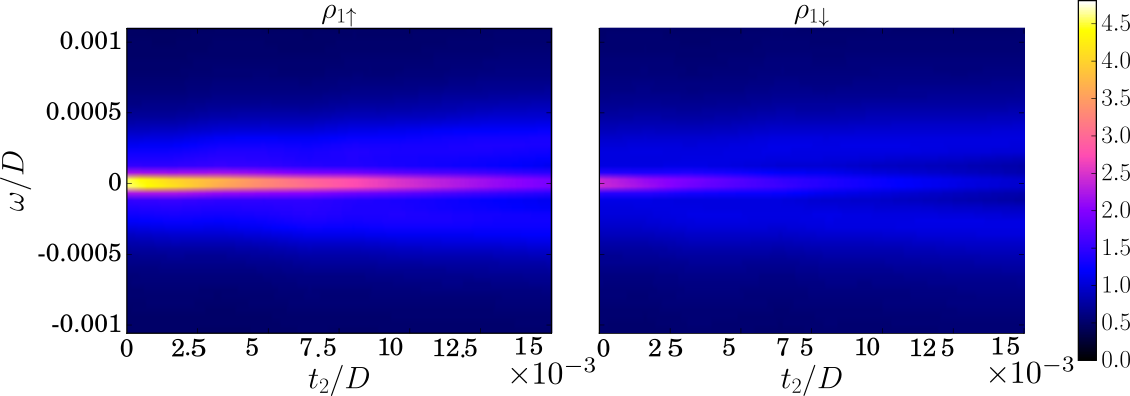
\includegraphics[scale=0.38]{Plots/2D/Shift_t2D1.png}
\caption{\label{fig:DOS/Shift_t2D1} Evolution of the DOS in the first QD }
\end{figure}
% \begin{figure}[hbt]
% \centering
% 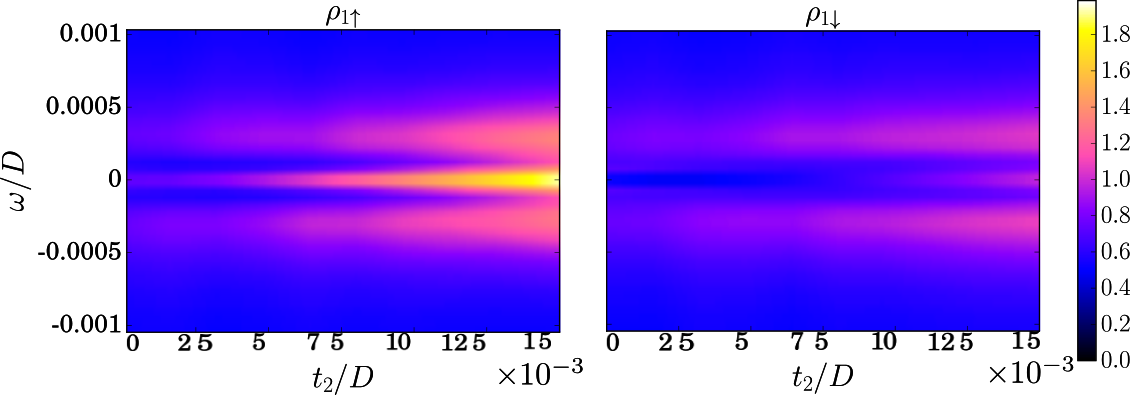
\includegraphics[scale=0.38]{Plots/2D/Shift_t2D2.png}
% \caption{\label{fig:DOS/Shift_t2D2} Evolution of the DOS in the Second QD}
% \end{figure}



\iffalse
\begin{figure}[hbt]
\centering
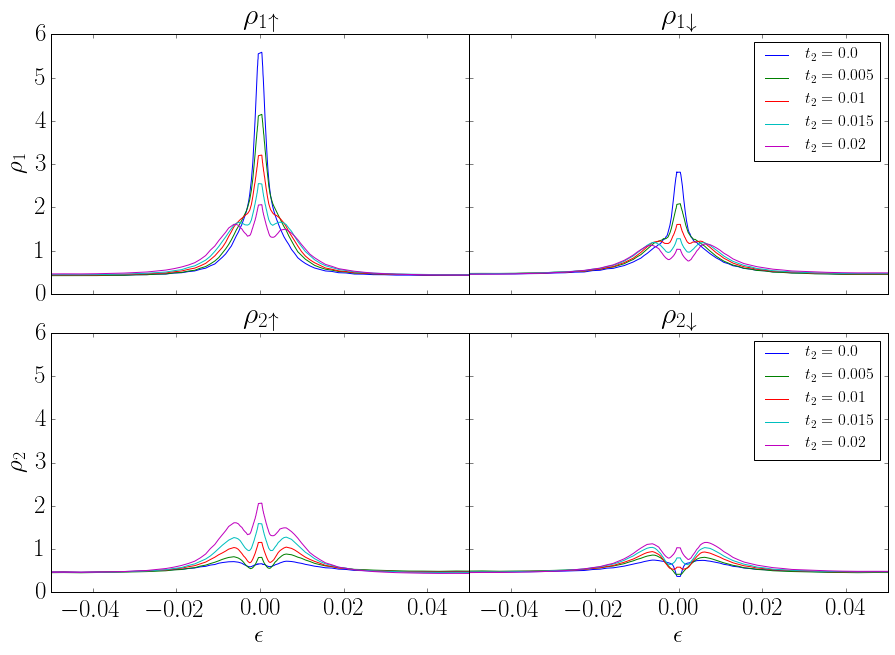
\includegraphics[scale=0.38]{Plots/DOS/Shift_t2.png}
\caption{\label{fig:DOS/Shift_t2} Evolution of the QDs' DOS for the procedure in \ref{fig:Mod/Shift_t2} }
\end{figure}
\fi
 In \ref{fig:DOS/Shift_t2D1} and \ref{fig:DOS/Shift_t2D1} we observe the evolution of DOS in the case where the second dot is smoothly connected to the Majorana, which is already attached to the first dot. The hopping parameter $t_2$ scales up to $0.015D$ where the model reaches the symmetry $t_2 = t_1$. The figures show that increasing $t_2$ leads to a drop in the DOS of QD1 while the DOS in QD2 is increased. In addition, the single peak in the first dot transforms into a three-peak due to the Majorana interference with the second dot. In \ref{fig:MSig/Shift_t2} we also observe that the reason between the zero up-down DOS  $\left(\frac{\rho_\up(0)}{\rho_\up(0)}\right)$ smoothly scales up to $2$ in QD2. At $t_2 =0.02$, when the  is completely symmetric, the Majorana signature appears in both quantum dots. Note that the relation $\frac{\rho_\up(0)}{\rho_\up(0)}$  is already close to $2$ at $t_2=0$. This implies that the second dot "feels" the Majorana even when it is not directly connected to the Majorana mode. 





